\Lecture{Jayalal Sarma}{September, 11 2015}{23}{General Graph Isomorphism}{Vidhya Ramaswamy}{$\beta$}{Ramya C}

\section{Introduction}
In these set of lectures, we consider the general graph isomorphism problem, and improve the solution. We know that we have a trivial solution in $O(n^n)$ time, by checking all possible mappings from graph $X_1$ to graph $X_2$. In the previous lecture, we have shown that when the graphs have a degree $d$ bound, we have an $O(n^{d^2})$ time solution.
\\We now give a $O(n^{n^{\frac{2}{3}}})$ bound for solving the general graph isomorphism problem.

\section{Colourings and Refinements of Colourings}
A colouring of a graph is a function mapping vertices of a graph to integers.
\[
f: V \longrightarrow \{1, 2, ... |V|\}
\]
To make understanding easier, we assume that $Range(f)$ is some initial segment of $\{1, 2, ... |V|\}$. That is, if we assign $k$ colours to all the vertices, we assume that the $k$ colours used are $\{1, 2, ... k\}$.
\paragraph*{}
We now introduce the idea of a Refinement of a Colouring. We can understand the idea of a refinement empirically as follows. Consider a colouring $f$ of a graph $X$. This partitions the graph into some colour classes. Now, we say that $g$ refines $f$ if $g$ further partitions each of these colour classes. 
\\Formally, we define refinement as follows:
\begin{definition}
We say that a colouring $f_1$ refines a colouring $f_2$ if $\forall x, y \in V$,
\[
f_2(x) \le f_2(y) \Rightarrow f_1(x) \le f_1(y)
\]  
\end{definition}
We write this as $f_1 \le f_2$
\section{Algorithm}

We notice that if we colour the graphs such that any isomorphism between the graphs would preserve the colouring, then, our job of finding an isomorphism becomes potentially easier, especially if each of the colour classes have very few vertices in them.
\paragraph*{}
We do this by choosing a colouring which preserves the degree information. 
\begin{enumerate}
\item Initially, all vertices are coloured with the same colour.
\item At each step, we refine this colouring, by encoding the number of vertices of a particular colour which are its neighbours. 
\item We continue this refinement process until no changes are made in the colouring. We call this a \textbf{stable colouring} of the graph.
\end{enumerate}
\paragraph*{}
Formally, we describe the refinement process as follows:\\
Let $f$ be a colouring, mapping a vertex $x$ to colour $f(x)$, using $k$ colour classes. Now, we describe $g$ (the refinement of $f$) as follows.
\begin{eqnarray*}
g(x) = (f(x), \chi_1(x), \chi_2(x), ... & \chi_k(x))
\end{eqnarray*}
where $\chi_i(x)$ = Number of neighbours of $x$ in colour class $i$.\\  
We can now order the tuples in some order (maybe lexicographic) and then map them to $\{1, 2, ... |V|\}$.\\
As we encode $f(x)$ in the beginning of $g$, $g$ is obviously a refinement of $f$.
\paragraph*{}
\begin{definition}
We say that 2 vertices are \textbf{not distinguished} if they are in the same colour class for a stable colouring.
\end{definition}
When we get a stable colouring, we observe the following:
\begin{observation}
For 2 vertices to be not distinguished, they have the same degree within each colour class. 
\end{observation}
\begin{observation}
When the colouring is stable, 
\begin{enumerate}
\item The induced graph of any colour class is regular.
\item The bipartite graph between any 2 colour classes is semi-regular. That is, each vertex in the left partition has the same degree, each vertex in the right partition has the same degree, but these degrees need not be the same.
\end{enumerate} 
\end{observation}

\textbf{Note: }If 2 vertices are not distinguished, this does \textbf{not} imply that an automorphism mapping one vertex to the other is possible. 
Consider figure \ref{fig:StableColouringNotIsomorphic6} below. As every vertex in this graph has a degree 3, the refinement process stops after one pass, and all vertices are coloured with the same colour.
However, there is no automorphism mapping vertex 1 to vertex 3.
\begin{figure}[htp!]
	\centering
	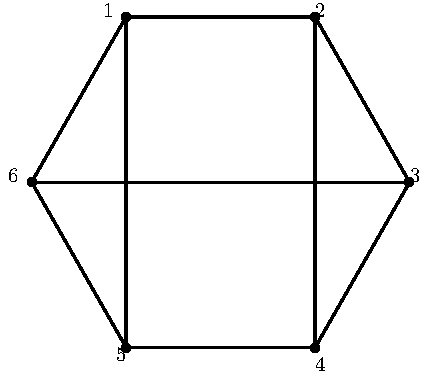
\includegraphics[scale=1]{images/not_iso.pdf}
	\caption{No automorphism mapping vertex 1 to 3}
	\label{fig:StableColouringNotIsomorphic6}
\end{figure}
\\We can also see an example where all vertices are in the same stable colour class, but there are no non-trivial isomorphisms (See \ref{fig:StableColouringNotIsomorphic12}) .
\begin{figure}[htp!]
	\centering
	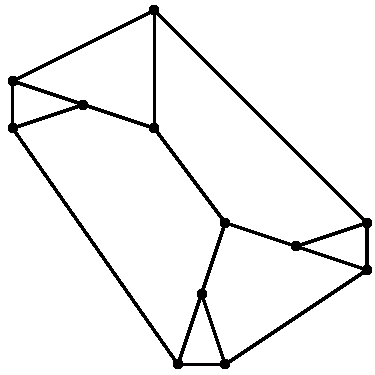
\includegraphics[scale=1]{images/not_iso12.pdf}
	\caption{No non-trivial automorphism}
	\label{fig:StableColouringNotIsomorphic12}
\end{figure}



\paragraph*{}
We claim that this process of refinement does not lose any isomorphisms. That is, 
\begin{claim}
If $f_1 \le f_2$, 
\[
(X_1, f_1) \cong (X_2, f_1) \Leftrightarrow (X_1, f_2) \cong (X_2, f_2)  
\]
\end{claim}
We leave the proof of this claim as an exercise to the reader.

\paragraph*{}
If, after obtaining a stable colouring, we have only one vertex in each colour class, we are done, as this forces each vertex to be mapped to a specific vertex in the other graph. 
If not, we force singleton colour classes by the idea of \textbf{Individualisation}.

\subsection{Individualisation}
For individualisation, we do the following.
\begin{enumerate}
\item Choose any vertex $x$ such that it is not in a singleton colour class, and colour it with a new colour.
\item Refine the colouring, until we get a stable colouring again. 
\item Repeat steps 1 and 2 until we get singleton colour classes.
\end{enumerate}
We notice that as soon as we start individualising vertices, we lose the property that the colouring preserves all isomorphisms, and hence, need to check it with all possible vertices in the corresponding colour class. In the next lecture, we look at how to pick these vertices to make our search smaller, and complete the proof of the general graph isomorphism.

\Lecture{Jayalal Sarma}{September, 14 2015}{24}{General Graph Isomorphism}{Vidhya Ramaswamy}{$\beta$}{K Dinesh}

\paragraph*{}
In order to decide which vertices of graph $X_1$ to individualise, we introduce the notion of \textbf{Colour Valence}.

\begin{definition}
Colour valence of a graph $X$ with a colouring $f$ is $d$, if, for every colour class $c$, and for every vertex $v \in V(X)$, there are atmost $d$ neighbours of $v$ in colour class $c$ or there are at most $d$ non-neighbours of $v$ in the colour class $c$
\end{definition}

Like having a bounded degree, having a bounded colour valence gives us an interesting bound on checking if 2 graphs are isomorphic.
\begin{claim}\label{ColourValenceD}
If $(X_1, f_1)$ and $(X_2, f_2)$ are given coloured graphs of colour valence at most $d$, then we can check if $(X_1, f_1) \cong (X_2, f_2)$ in time $O(n^{d^2})$.
\end{claim}

Hence, if we can get a colouring of both graphs which preserves isomorphisms, and is of a constant colour valence, we can use the above claim (Claim \ref{ColourValenceD}) to check if the graphs are isomorphic in polynomial time. 
To do this, we need to ensure that when we individualise vertices, we reduce the colour degree. The following lemma allows us to do so.

\begin{lemma} \label{PickVertexIndividualisation}
Given a coloured graph $(X, f)$ with a colour valence less than or equal to $d$, we can find vertices $x_1, x_2, ... x_k$ where $k \le \frac{2n}{d}$, such that $(X, f')$ has a colour valence $\le \frac{d}{2}$ where $f'$ is the stable colouring obtained by individualising $(X,f)$ on vertices $x_1, x_2, ... x_k$.
\end{lemma}  

Assuming Claim \ref{ColourValenceD} and Lemma \ref{PickVertexIndividualisation}, we get algorithm \ref{GeneralGI}.

\begin{algorithm}[htp!]
\caption{Algorithm for general GI}\label{GeneralGI}
\label{alg:generalGI}
\begin{algorithmic}[1]
\Procedure{General GI}{ Input : Graphs $X_1, X_2$ }
\State Given $X_1, X_2$
\State Start with a trivial colouring of $X_1$ and $X_2$. Refine until stable.
\State Choose $(x_1, x_2, ...x_k)_{\log n}$ according to Lemma \ref{PickVertexIndividualisation} for $X_1$. This gives us a colouring with colour valence as some constant.
\For {$(x_1, x_2, ...x_k)_{\log n}$ in graph $X_2$}
	\If {Colour valence of $X_2$ is not a constant}
		\State \textbf{break}
	\Else
		\State Use claim \ref{ColourValenceD} to check if $X_1$ and $X_2$ is isomorphic.
		\State If so, output that $X_1 \cong X_2$.
	\EndIf
\EndFor
\State Output that $X_1 \not \cong X_2$
\EndProcedure
\end{algorithmic}
\end{algorithm}

Hence, we have an algorithm for graph isomorphism, modulo the proofs of Claim \ref{ColourValenceD} and Lemma \ref{PickVertexIndividualisation}.
\paragraph*{}
\textbf{Proof of Lemma \ref{PickVertexIndividualisation}}
\begin{proof}
Let $S$ be a a set of vertices chosen upto stage $i$, that is, $S = \lbrace x_1, x_2, ... x_{i-1} \rbrace$. Let the colouring after these individualisations be $f_S$.
Since we are not yet done, colour valence of $(X, f_s) > \frac{d}{2}$.

Therefore, $\exists$ a colour $m$, and a vertex $x \in V(X)$ such that
\[
d_m (x) > \frac{d}{2}
\]
and 
\[
cod_m (x) > \frac{d}{2}
\]
where $d_m(x)$ is the number of neighbours of $x$ in colour class $f_S^{-1}(m)$, and $cod_m(x)$ is the number of non-neighbours of $x$ in colour class $f_S^{-1}(m)$.
We make the following claim:
\begin{claim}\label{NeighboursNonIntersect}
We can choose an $x_i$ such that $x_i$ violates the colour valence property, and,  
$\forall j < i$
\[
N(x_i) \cap N(x_j) = \phi 
\]
where $N(x)$ is the neighbour set of a vertex $x$ in $X$.
\end{claim}
Choosing $x_i$'s as per claim \ref{NeighboursNonIntersect} suffices. We can sum up the neighbours of all these $x_i$'s, and get the following inequalities:
\[
\frac{kd}{2} \le \sum_{j=1}^k |N(x_j)| \le n
\] 
Hence, we get 
\[
k \le \frac{2n}{d}
\]
\end{proof}

We still need to prove claims \ref{ColourValenceD} and \ref{NeighboursNonIntersect}.
